\documentclass[11pt,a4paper,final,notitlepage]{report}
\usepackage[utf8]{inputenc}
\usepackage{amsmath}
\usepackage{amsfonts}
\usepackage{amssymb}
\usepackage{fullpage}
\usepackage{graphicx}
\usepackage{grffile}
\usepackage{url}
\usepackage{enumitem}
\usepackage{xcolor}
\usepackage{textcomp}
\usepackage{listings}
\usepackage{varwidth}
\usepackage{hyperref}

\usepackage{caption}
\usepackage{subcaption}

\usepackage{stackengine,graphicx,trimclip,scalerel}


\renewcommand{\baselinestretch}{1.25} %Increase 

\makeatletter
\newcommand*{\toccontents}{\@starttoc{toc}}
\makeatother

\newcommand{\noNumberChapter}[2]{
    \setcounter{chapter}{#1}
    \setcounter{section}{0}
    \chapter*{#2}
    \addcontentsline{toc}{chapter}{#2}
}

\usepackage[nopar]{lipsum}
\usepackage{stackengine,graphicx,trimclip,scalerel}
\savestack\eye{\rotatebox{90}{$^\circ\mkern-6mu\raisebox{1pt}{)}$}}
\savestack\nose{\raisebox{3pt}{\scalebox{1}[-1]{\clipbox{0pt 1pt 0pt 0pt}{?}}}}
\savestack\mouth{\rotatebox{90}{(}}
\newcommand\Lenny{(\scalerel{\stackanchor[2pt]{\eye \nose \eye}{\mouth}}{)}}




\begin{document}

\title{ Major Project Report }

\author{ Tom Minor - Level H\\
 		 Major Project\\
 		 Bournemouth University, NCCA\\
 		 \\
 		 Supervised by Oleg Fryazinov, Adam Redford
		}

% Remove date
\date{}
\maketitle

\renewcommand{\abstractname}{Project Overview and Responsibilities}
%\\We have crazy integration, crazy asset production, crazy pipeline and our own GPU renderer - that's quite cool when you put it that way
\begin{abstract}

\begin{center}
\begin{varwidth}{\textwidth}
\begin{enumerate}
\item Fractal Renderer
\item FX
\item Pipeline\\
\end{enumerate}
\end{varwidth}
\end{center}

\textbf{CONTACT} is a near 3 minute long VFX sci-fi short, showing an astronaut’s state of mental decay after experiencing an encounter with a 5th dimensional being while in orbit. The team worked hard to create over 80 CG assets, 3 digital environments, and a bespoke fractal render engine for the evolving tunnel sequence at the height of the piece. Over 26 shots were composited into these built environments and costumes, fleshing out the narrative and blending together the live-action and the digital elements of the film.

\end{abstract}

\toccontents

\chapter{Introduction}
I originally planned to create a Fractal LookDev Tool by creating my own renderer and working alone on an R\&D project, as pathtracing and fractals are a combination that I really find fascinating. However, after talking to Kyran Bishop we both came up with an initial pitch strongly inspired by the film A Space Odyssey \cite{hal} that culminates in a dramatic psychedelic sequence. This gave me a fantastic opportunity to develop a fractal tool that would actually be put to the test by a team of artists and be integrated in a piece to create something visually stunning. 

As an R\&D technical person, it is always more satisfying and gratifying to create a tool with an actual purpose that will be used by other people. Joining a team of artists made my overall job harder as the result had to be absolutely polished and of professional quality which really pushed me to develop the tool the best I could. Within the group, I set out initially to work on the renderer alone but given the large amount of work we had to do as a group it was unrealistic to expect myself to work purely on that. This meant I took up additional roles such as Pipeline TD and wrote a plugin that encompasses Perforce in Maya as this only existed for Windows and not Linux, and FX TD to create a destruction effect for our piece.

\chapter{Initial Research}

\section{Fractal Sequence}
\subsection{Fractals in FX Software}

It would have made no sense to go ahead with the fractal tool idea if it was easily possible in existing renderers, initially I looked into developing fractals in Houdini. The most common approach for the Mandelbulb  fractal shape I was focusing on was to calculate the voxel based shape and render it was a volume, The results were quite sucessful \ref{fig:voxelbulb} and while this did give an effect similiar to that achieved by Disney in the Big Hero 6 \cite{bh6} fractal sequence, it was far too slow to compute for any form of interactive tweaking to be used for our fractal sequence that would need several hundred frames rendered. 

After a little more research, I found out faster alternatives in Houdini created by the FX team responsible for the fractal sequence in \textit{Lucy}. They implemented a Vex based raymarcher \cite{Kim:2014:CIU:2614106.2614166} that worked and rendered a lot  faster than a volumetric approach, but it still suffered from interactivity issues that specialised solutions like Shadertoy do not. 

I decided Houdini wasn't the way to go for developing my tool but still used it several times during the project for several other tasks such as some creature FX R\&D work  \ref{fig:noise_shader} and Voyager destruction. Shadertoy and GPU Accelerated rendering of implicit surfaces seemed to be the efficient way of rendering, so I began moving in that direction for creating my custom lookdev tool.

\begin{figure}
\begin{center}
\includegraphics[scale=0.2]{"images/houdini_mandelbulb"}
\caption{Voxel Based Volumetric Mandelbulb}
\label{fig:voxelbulb}
\end{center}
\end{figure}

\begin{figure}
\begin{center}
\includegraphics[scale=0.2]{"images/noise_shader"}
\caption{Houdini Plasma Shader Effect}
\label{fig:noise_shader}
\end{center}
\end{figure}


\subsection{Distance Estimated Fractals}


\begin{figure}
\begin{center}
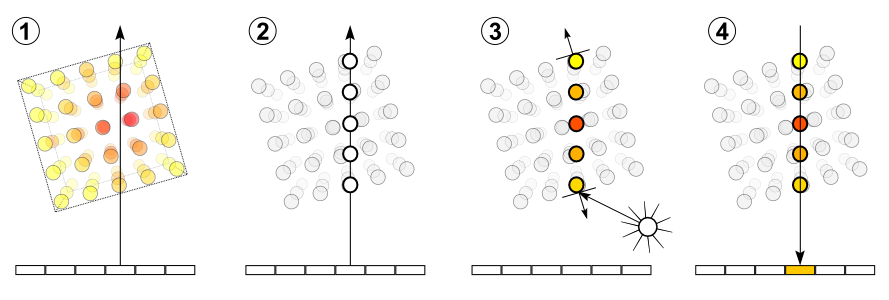
\includegraphics[width=\textwidth]{images/raymarchstep}
\caption{Ray marching algorithm}
\label{fig:raymarching}
\end{center}
\end{figure}

The basic raymarching algorithm can be optimised through a technique known as Sphere Tracing \cite{Hart1996}, which requires knowing the nearest distance to a surface at any point \ref{fig:sphere_tracing}. A function known as a distance estimator can be used to find this distance, which makes the basic process becomes something like 

\begin{figure}
\begin{center}
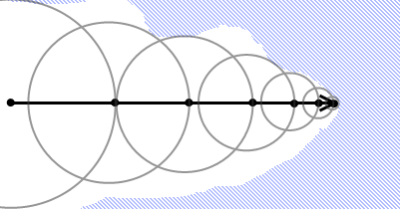
\includegraphics[width=\textwidth]{images/spheretracing}
\caption{Sphere tracing algorithm}
\label{fig:sphere_tracing}
\end{center}
\end{figure}



\subsection{Raymarching in a shader}

As a proof of concept, I created a Qt project that drew a fullscreen quad onscreen. I then experimented with the GLSL shader to try and recreate Shadertoy myself, this was the result:

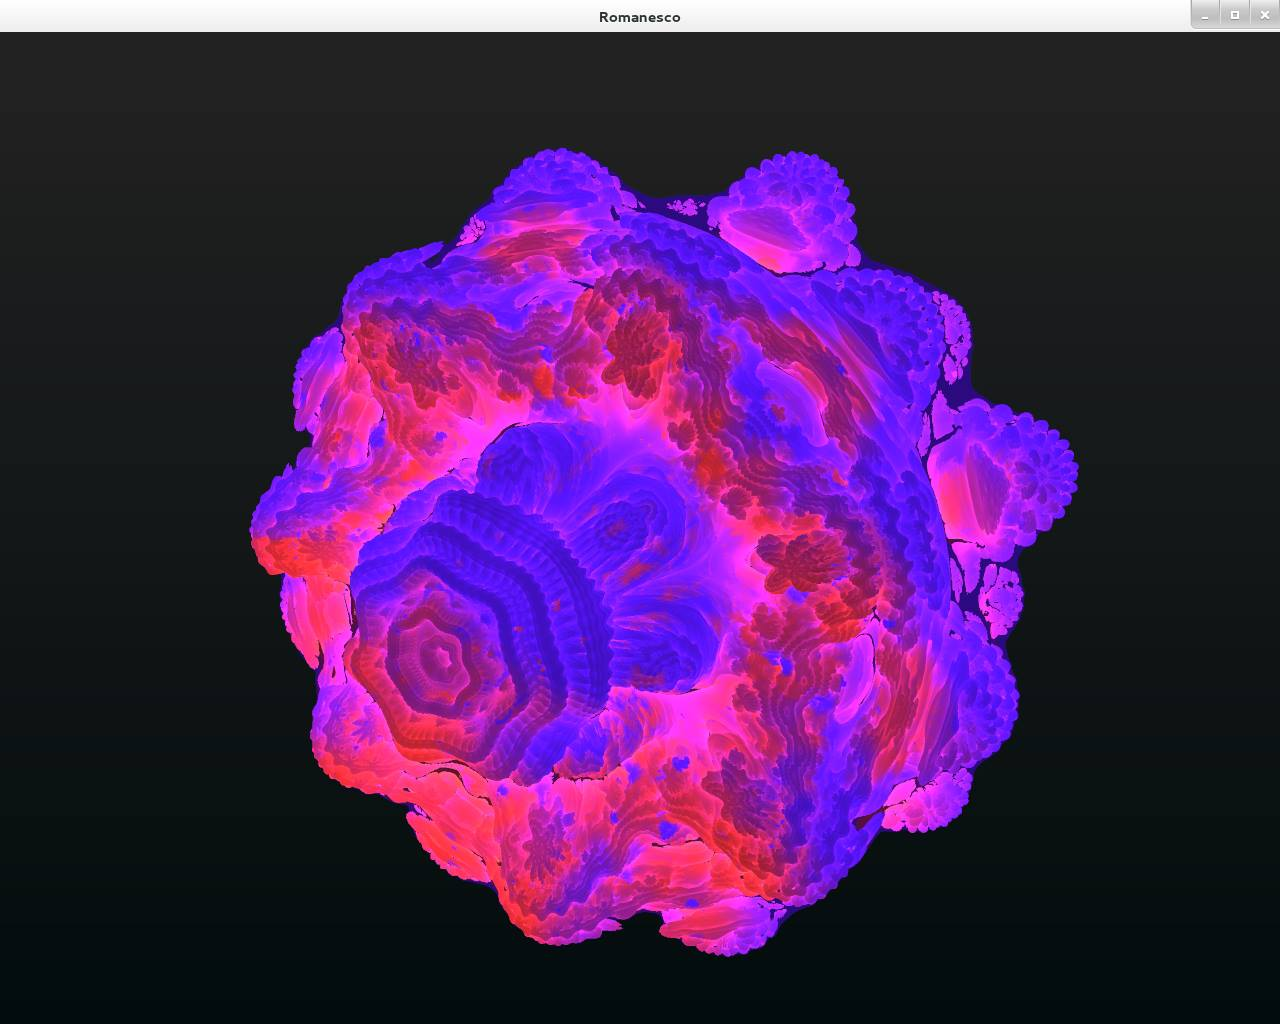
\includegraphics[width=\textwidth]{images/gl_bulb}






\chapter{Fractal Sequence}

Armed with the knowledge that raymarching in a shader is the way to go, I looked into writing my renderer in CUDA for more control. I soon found out that NVIDIA Optix would be a much better choice, as it does a lot of the difficult work like ray batching for me but is still highly programmable.

\section{Romanesco (Fractal Tool) Requirements}

Initially, I wanted the tool to be used by the rest of the team, so my requirements were more in line with usability. However I needed to get visuals out of it as soon as possible, so this was put on the backburner while I worked on getting the rendering component working.

\section{Rendering Strategy}
The world is rendered using a simple pinhole camera \cite{pinhole}. To get realistic lighting I decided to implement path tracing \ref{fig:path_tracing}, this was completed late in the project and is not the most efficient lighting algorithm. This is just because of how path tracing works, as rays hit geometry in the scene many more rays are recursively bounced around the scene. However, given the rendering speed of the frames thanks to the GPU even HD renders don't take long to complete.

Progressive rendering and path tracing go hand in hand, so this was a natural progression of that. It allows the user to work in a preview mode with very noisy lighting that is fast, while still allowing the samples to be pushed up for renders where interactivity isn't as important.


\begin{figure}
\begin{center}
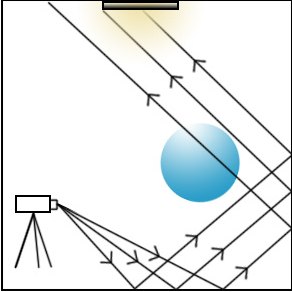
\includegraphics[scale=0.5]{images/pathtracing}
\caption{The path tracing process}
\label{fig:path_tracing}
\end{center}
\end{figure}


I ran into issues while rendering large frames with many samples per pixel however, especially on slower GPUs. This was because the kernel launch would timeout if the calculations took too long. An elegant solution was to make use of tile based rendering \cite[pp. 51-52]{kalamp}, which basically cuts up the image into multiple chunks of tiles which then get rendered one by one in a serial fashion. There is an overhead in launching an Optix render multiple times per frame instead of once, but it is not as intrusive as a full crash that would occur in a timeout. It also has the potential to simplify implementation of other rendering algorithms in the future, for example Bidirectional Path Tracing stores light paths in an array that can become very large for huge images but is manageable for small tiles.

\section{Output}
In order to be useful in a VFX scenario I need to at least output channels such as normal, position and depth. Additional channels such as iteration count are also useful.

To achieve this, the Optix shading programs are setup to write to predefined buffer layouts. This does make it tedious to extend with new channels when needed, but it is unlikely to change often. When an EXR file is saved (using OpenImageIO), I load in the data from all the Optix buffers into the appropriate EXR channel. This data can then be accessed in Nuke for compositing work. \ref{fig:exr}

One potential issue that was fixed was compression, I knew we needed to render 650 1080p frames at some point and with 6 channels worth of data in each that would rapidly eat up disk space. The elegant fix to this was to turn on ZIP compression in the EXR spec before saving.

\begin{figure}[h!]
	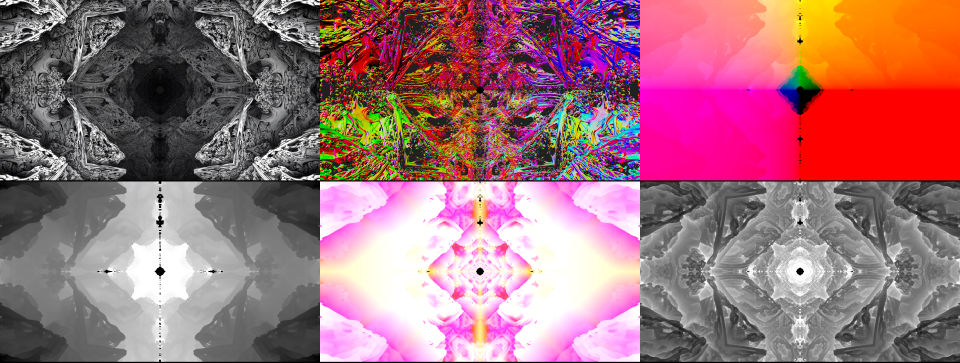
\includegraphics[width=\textwidth]{images/contactsheet}
	\caption{A contact sheet of all the EXR passes exported from the renderer}
	\label{fig:exr}
\end{figure}


\subsection{Environment Camera}
Although it was a last minute request, getting an environment camera working was vital for relighting the astronaut. I fixed it quickly to avoid holding back production, and thankfully the way I setup the various buffers maps directly onto the new camera model with no modification, adding the camera was as simple as defining a new ray generation program.

This means that EXRs can be rendered with either the pinhole or environment camera and they will have identical data passes, this allowed us to use the exact same compositing networks to calculate the environment colour and have a 1:1 match for the relighting of the astronaut. Nuke and Maya accept the generated maps as environment maps with no issues.

\begin{figure}
\begin{center}
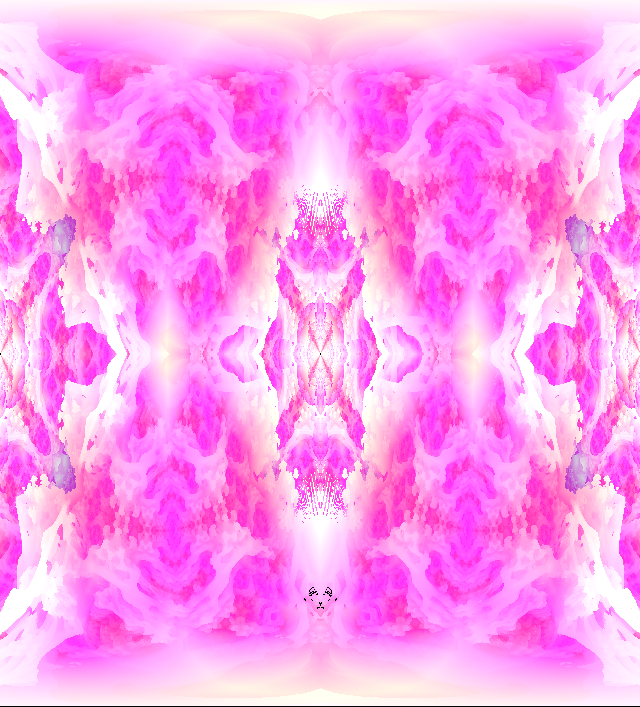
\includegraphics[scale=0.5]{images/orbitenv}
\caption{An environment map render with the orbit trap pass visible}
\label{fig:path_tracing}
\end{center}
\end{figure}


\section{Colouring the fractal consistently}

A major issue we ran into during production was colouring the fractals, initially comp only tests were attempted but they didn't work very well because the form changes so rapidly.

Iteration count would work as a basic 0-1 range that can be used to remap some colour ramp onto it, but the result is very boring and doesn't have any fractal qualities.

The solution was orbit traps, where by the value given is determined by how close the fractal iterative function approaches a chosen shape. Although we not limited by the type of orbit traps we can use, I didn't have time to research much beyond the examples I found people using on shadertoy.

In the current shot setup there are three types of orbit traps employed:
\begin{enumerate}
	\item A spherical orbit trap that stays consistent as the shape changes
	\item Another spherical trap, except as the iteration count gets deeper the size of the sphere it is trapping gets smaller.
	\item A tube orbit trap that produces interesting spots and 'petals' across the shape
\end{enumerate}

These orbit traps are encoded in the orbit.RGB channels of the EXR pass. This was configurable on a per scene basis if necessary (in the case of the tunnel scenes it was, the tube orbit trap gave useless values and needed manual tweaking)

Although the colours straight out of the render are odd looking, the values are intended more as a data pass to drive more complex recolouring setups.


\section{Scene Management}
In an effort to get everything working on time, I ended up having to fallback to simpler ways of saving the scene. If I were to use a nodegraph, I'd have to wrestle with JSON or XML files, but at this stage I simply decided to save the scenes as .cu files containing CUDA hit functions. The camera information is encoded in the comments at the top of the file, for example
\begin{lstlisting}
// 0 34 0
// 1.5 0 1.3
// 30
\end{lstlisting}

Would start the camera at (0,34,0), rotated by (1.5, 0, 1.3) with an FOV of 30.

These scenes are compiled at runtime using code reflection techniques.

\subsection{Code Reflection}
Runtime compilation is necessary for allowing scene changes at runtime, specifically the ability to compile to .ptx code so it can be loaded into Optix as a callable function.
\subsubsection{Methods}

\begin{itemize}
	\item NVRTC - Available in CUDA 6.5 and up, faster and built in way of compiling.
	\item System NVCC - If using an older version of CUDA (such as on the university lab workstations), I try to use the system NVCC (hopefully available in path). This has the downsides of requiring the developer tools to be installed, as well as the performance overhead of launching and managing a subprocess. However, this allows me to render on a wider range of machines regardless of the performance impact.
\end{itemize}

\subsection{Runtime Patching}
Once the code is compiled, I needed some way to tell Optix to use it.

\subsubsection{PTX Patching}
		\begin{itemize}
			\item My initial attempt, required research into the .ptx format.
			\item Use NVCC to compile CUDA program into ptx code and patch into the Optix ptx code, then load into Optix
			\item Works on my machine and university workstations, but potentially undefined behaviour and not officially supported
			\item Relies on my own string handling functions
			\item Manually patching the generated PTX code ( prone to error )
		\end{itemize}



\subsubsection{Optix Callable Programs}

\begin{itemize}
			\item Discovered this later in the project after reading the Optix documentation fully, initially didn't notice what it was because it's not used very often compared to the other aspects of optix and isn't really clear unless you know what it does.
			\item Use NVCC to compile CUDA program into ptx code and then tell Optix to use this as a 'callable program', basically replacing the ptx patching process with a well defined, built in functionality.
				\item Optix rtCallablePrograms ( officially supported way of doing it, found out later in the development process )
			
\end{itemize}

\subsection{Node Graph}
An alternative to the TD style CUDA 'scene file' approach is to use a node graph to replace it's functionality. This has a number of benefits for the artist and was my original plan, but had to be abandoned due to time constraints. 

It influenced the current design, which is a simplified form of what the node graph would have been.

\subsubsection{Grammar Definition}
In order to properly write a parser for the node graph, it was important to treat the node graph like a simple language. This was helpful in figuring out error conditions, for example if a domain operation is plugged into a distance operation \ref{fig:grammar}

\begin{figure}[h!]
	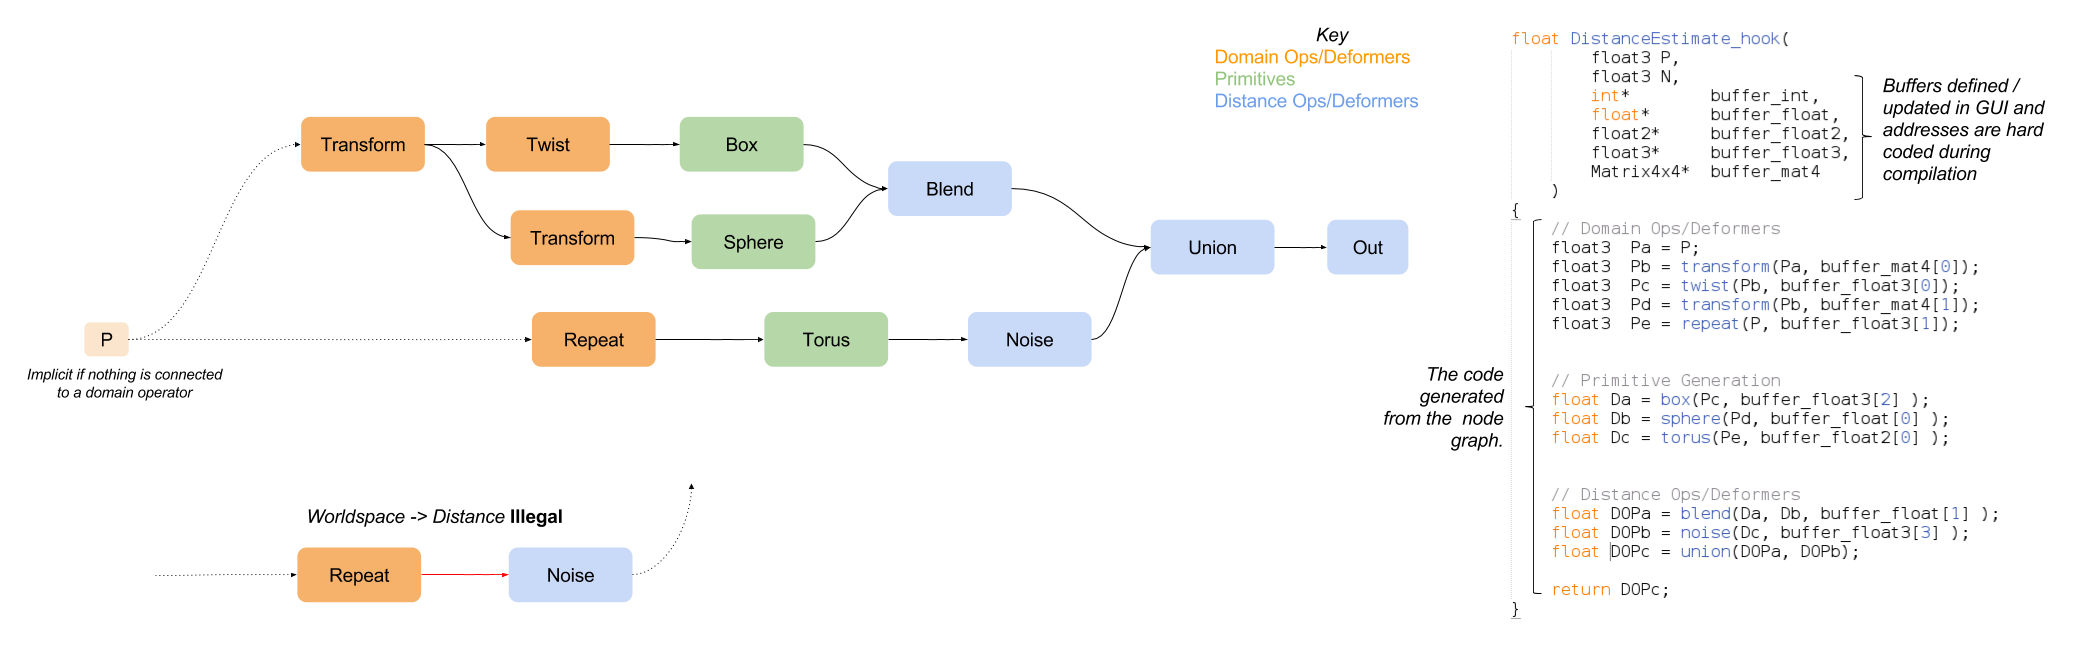
\includegraphics[scale=0.25]{nodegrammar}
	\caption{My Nodegraph Grammar Definition}
	\label{fig:grammar}
\end{figure}



\section{How the Shots were achieved}
\subsection{Side Sequence}

The side sequence was much simpler compared to the tunnel shot, as it didn't even require a complex new fractal in the end. I realised that the Mandelbulb's pole looks like a chomping 'maw' as the powers increase, so the effect basically consists of the bulb's power slowly morphing from 2 through to 5 as the scene goes on. This also helps create the effect that the shape is growing.

To physically move the shape towards the astronaut, I simply applied a scene wide transformation that moves the Mandelbulb along the Z axis. Another transform slowly rotates it around the Z axis too.

Finally, a low FOV of 30 helps give the impression that the shape is huge.

\subsection{Tunnel Sequence}

\begin{figure}
\centering
\begin{subfigure}{.5\textwidth}
  \centering
  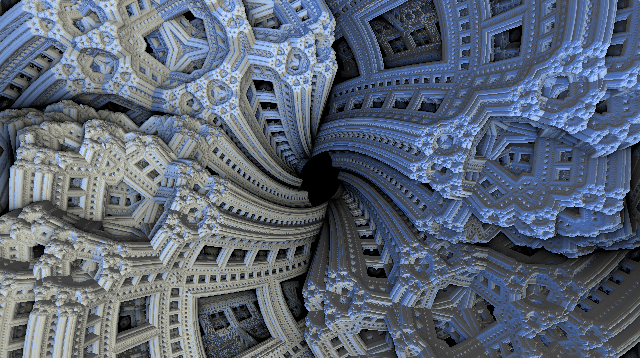
\includegraphics[width=.95\linewidth]{images/mengerjourney.png}
  \caption{Menger Journey \cite{mengerjourney}}
  \label{fig:menger}
\end{subfigure}%
\begin{subfigure}{.5\textwidth}
  \centering
  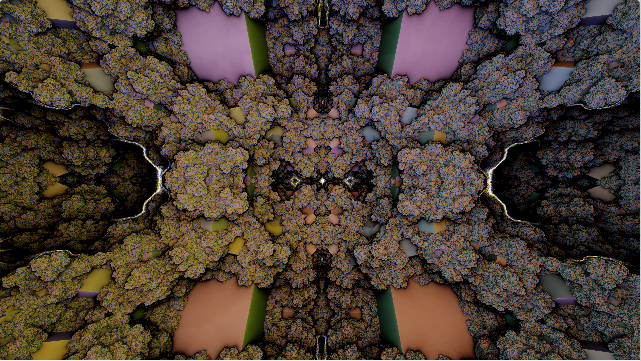
\includegraphics[width=.95\linewidth]{images/kaljourney.png}
  \caption{Kaleidoscopic Journey \cite{kaljourney}}
  \label{fig:kal}
\end{subfigure}
\caption{Two tunnel variations created by Syntopia, on Shadertoy}
\label{fig:test}
\end{figure}

The main tunnel shape was originally less organic, the base shape was heavily inspired by the work of Syntopia's Shadertoy demos \cite{mengerjourney} \cite{kaljourney}. 

My initial design was prototyped in shadertoy under the assumption I would port it over to the renderer, this prototype is visible here: \url{www.shadertoy.com/view/ls3SRs} \ref{fig:shadertoy}. However, due to team feedback the design changed dramatically and only some elements survived into the iteration shown in \ref{fig:initialdesign}.


The main desire of the team was to maintain symmetry, which disallowed the use of the twist effect that created such interesting motion in the Shadertoy iteration. However, I took some more inspiration from \ref{fig:kal} and applied the base shape to my IFS fractal, this created a very interesting pulsing and rotating motion that everyone liked. We were planning to use this in the final cut, but then I dug deeper into the workings of \ref{fig:kal} and discovered how the interesting surface details are created using \textit{geometry traps}.

\ref{fig:finaldesign} shows the result of applying a Mandelbulb geometry trap to the shape of the original IFS tunnel, because it is simply stuck to the surface it follows the interesting rotating motion of the tunnel but has the organic surface of a bulb.

\begin{figure}
\begin{center}
  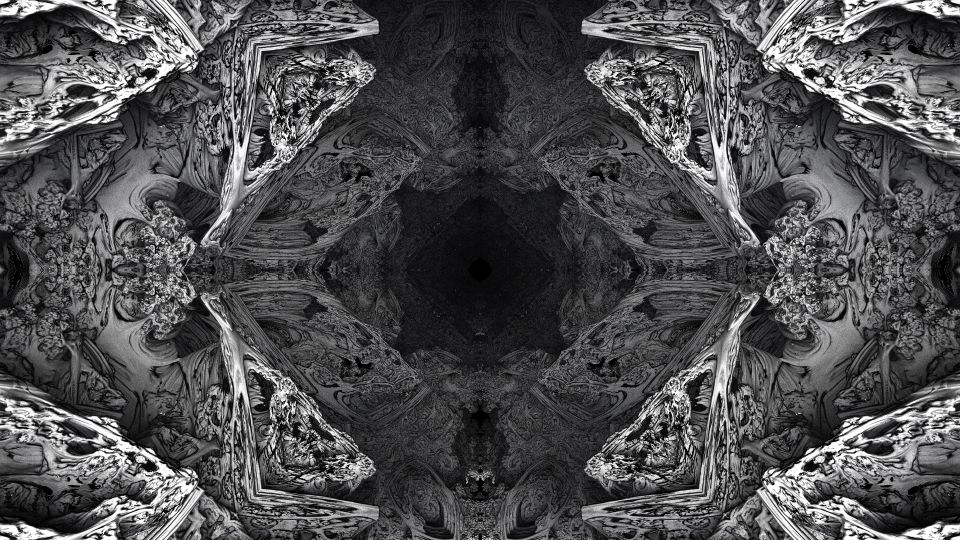
\includegraphics[width=.95\linewidth]{images/tunnelbulb.png}
  \caption{The final design}
  \label{fig:finaldesign}
\end{center}
\end{figure}


\begin{figure}
\centering
\begin{subfigure}{.5\textwidth}
  \centering
  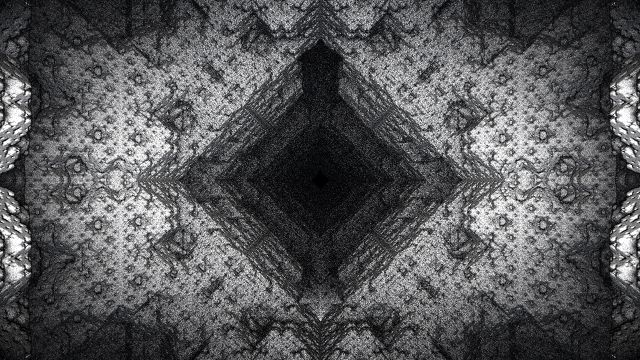
\includegraphics[width=.95\linewidth]{images/ifs_tunnel.png}
  \caption{The initial design}
  \label{fig:initialdesign}
\end{subfigure}%
\begin{subfigure}{.5\textwidth}
  \centering
  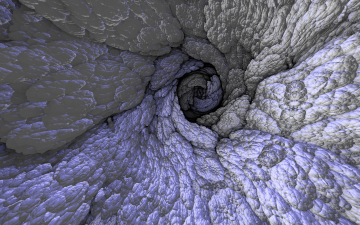
\includegraphics[width=\textwidth]{images/shadertoy_test}
\caption{Shadertoy Prototype}
\label{fig:shadertoy}
\end{subfigure}
\caption{Tunnel Iterations for the piece}
\label{fig:test}
\end{figure}

\subsection{Reflected Visor Sequence}
This one was done last

\begin{itemize}
\item Power 5 mandelbulb constrained within a manually tweaked box shape (via intersection function)
to cut off the majority of it’s mass and keep it’s shape light and tendril like
\item This entire shape is then intersected with the tunnel shape, combining the organic shape of
the Mandelbulb with the hole in the tunnel. This creates an interesting silhouette.
\item Primarily used as a silhouette in the comp, so not many samples were required for usable
frames.
\item A high FOV of 110 is used to stretch out the shape even more and ease the process of mapping
it onto the visor.
\end{itemize}

\chapter{Future Improvements}

\begin{itemize}
	\item Look into methods besides distance estimation for more fractal possibilities, brute force approach
	\item Make the interface more artist friendly, with less reliance on understanding the maths
	\item Improve the input handling and allow for multiple input methods such as gamepads
	\item Some form of adaptive rendering to keep the viewport responsive
	\item Improve the light sampling algorithms using methods such as Bidirectional Path Tracing, VCM or Metropolis light transport.
	\item Provide a GUI interface for the lighting setup
	\item Move the batch rendering script's capabilities directly into the main renderer
	\item Screenspace CUDA shaders that make use of the various buffers available	
\end{itemize}





\chapter{Dynamics FX}

For the voyager sequence I had to create the effect of debris slowly drifting through space, so created the genesis of the destruction sequence as a base of the effect.

\section{Setting up the simulation process}
\begin{itemize}
	\item Import the Voyager model as an FBX (with UVs) and convert the Maya hierarchy setup to Houdini groups
	\item Fracture a slightly pre-deformed version of the mesh, transfer the UVs and create new ones in the gaps
	\item Generate constraints between all nearby fractured pieces
	\item Manually paint on the strengths of each fractured piece, this is done by painting the strength onto the vertices and then finding the average strength of each fractured piece's vertices
	\item The core unit of voyager has a very high strength so it does not fall apart, as it has to be intact for the shot
	\item The manually painted strength values are multiplied by noise to get more variation
	\item The strength values are remapped using a curve for a less linear falloff
	\item Finally, transfer the strength values to the constraints and feed into the simulation
\end{itemize}

\section{Simulation Elements}
\begin{itemize}
	\item Fractured voyager with constraints
	\item Phantom collision geometry that initiates the destruction effect
	\item Zero gravity simulation, with torque and spin POP nodes to introduce interesting rotations into the simulation.
\end{itemize}

\section{Final Touches}
In the end, the simulation was exported to an alembic cache and Lewis processed it with a simple script that baked the animation data into locators. Using this method, we preserved animation ability for individual pieces if necessary but otherwise the simulation looked identical. Slowing down the simulation 20x in the Alembic's time scale was sufficient to give a convincing effect that the debris was slowly drifting, without completely stopping the simulation.



\chapter{Pipeline}

I decided to develop a strong pipeline at the beginning of the year because I felt with such an ambitious project a simple Dropbox pipeline would run into many probles. Given our needs, I decided to choose Perforce as it is capable of versioning binary files efficiently and it has built in mechanisms to prevent team members from accidentally overwriting each others work.

The first few months were spent learning how Perforce works, then learning it's Python API before finally figuring out the best ways to expose this in a GUI.
The initial effort was worth it in the end, as many times during the project files were randomly corrupted or work would have been overwritten if we hadn't decided to take the chance and use version control.

I spent a short while developing a Perforce wrapper for Maya using Python, Pyside and P4Python. None of the dependencies are platform or program specific, and in theory could allow the plugin to work not just in Maya but Nuke, Mari or anywhere that has Pyside available (with a few tweaks). It is also crossplatform and should work on Windows/Mac/Linux with little modification.

The end result is a pipeline suite in addition to the Perforce tools, it provides:
\begin{itemize}
	\item Asset version control and offsite backup on a remote server I configured to run Perforce (located on \textit{Amazon Web Services}).
	\item Changelist management.
	\item GUI ability to check out files and submit changelists.
	\item Preview an old file revision directly in maya with one button click.
	\item Revert to old revisions if necessary.
	\item Shot and asset wizards to automatically generate the folder. structures required by the pipeline that are tedious to do by hand.
	\item Student popup removal on save.
	\item Automatically makes any references relative to the \$CONTACTROOT environment variable, which was a necessary fix to work around our folder structure's limitations and worked well in the end.
\end{itemize}

Besides being a tool, it also changed the teams workflow. At the start of the year it was normal for people to get confused and try to edit the same file, despite Perforce preventing it. Now that never happens, as the team dynamic has changed to accommodate a more careful workflow.

There is also a lot of server side data that could have been used to analyse how the group was working, how much work was being done and by who, etc. We didn't approach this area as it could encourage faking work to look good, but the fact that the logs are available is a handy thing to have. 

\begin{figure}[h!]
	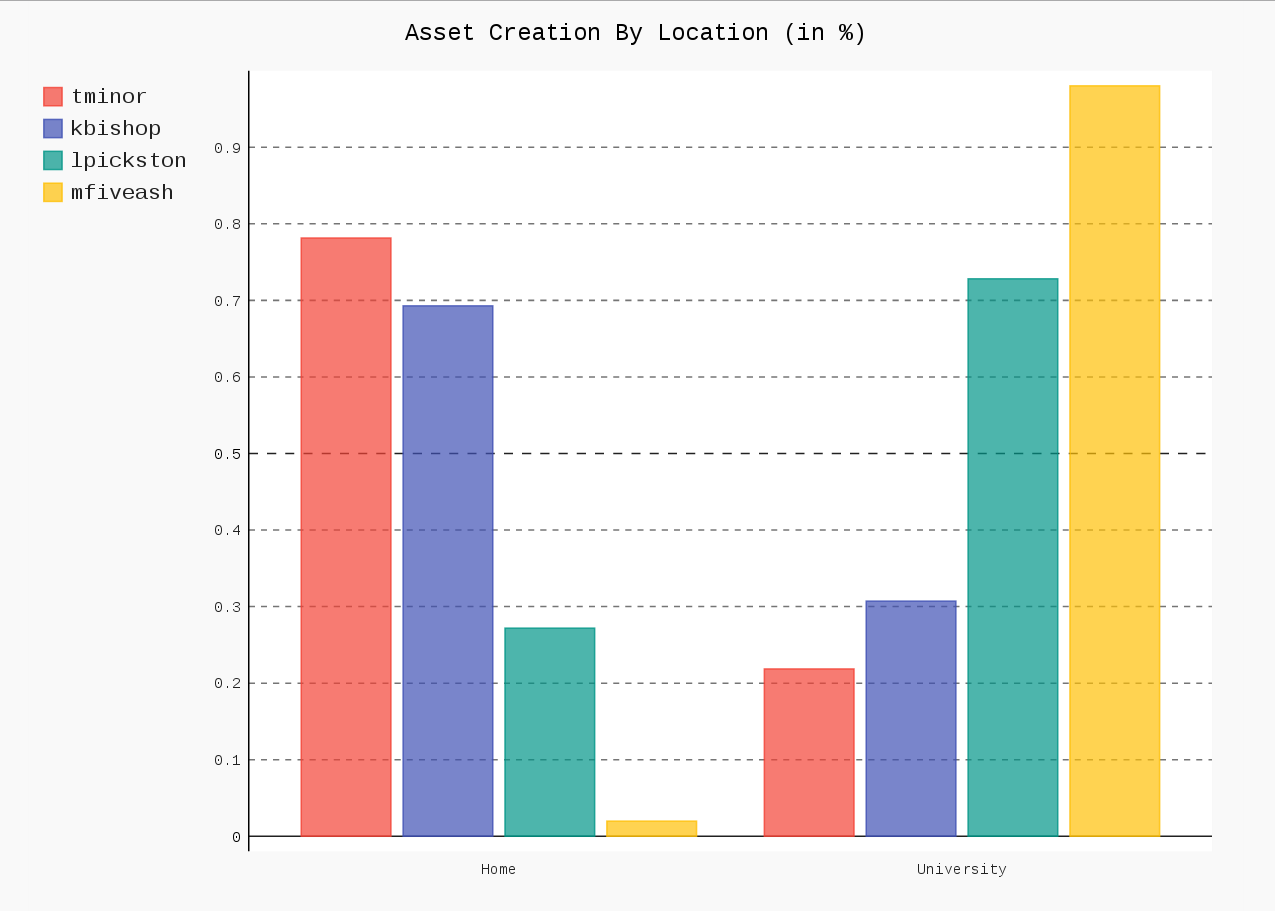
\includegraphics[width=\textwidth]{images/graph.png}
	\caption{Analytics generated with my python script to see how useful the log data is}
	\label{fig:graph}
\end{figure}



\chapter{Conclusion}

\paragraph{In conclusion} I believe Romanesco is a useful and novel way of developing fractal objects in a visual effects context. The majority of currently available renderers are more of a novelty, designed to create nice images for a desktop background instead of a usable plate. Attempting to use existing renderers to create fractals is a plausible method, but suffers from poor interactivity due to long calculation times for the fractal structure.

Romanesco begins to fill in the gap between the currently available approaches, with more polish and focus put towards artist usability the more important issues such as fractals not behaving well enough for real world VFX shots can be minimised by the ease in which it is possible to iterate on the fractal design using the renderer.

Despite the final result being a fairly technical tool to use, the artistic feedback from the rest of the team has been vital in getting it to this stage. If I had decided to do this project solo, I don't believe it would have developed beyond the tech demo stage. By having a strong team surrounding me, especially in the compositing department, I saw first hand which features were actually important instead of focusing on the ones that I personally had an interest in. In the end, this is the reason we ended up with 600 frames worth of fractal sequence that was successfully used in integration with a live action piece.
%========================================================


\nocite{*}

\bibliographystyle{plain-annote}
\bibliography{bib_icereport}
\end{document}
